\documentclass{article}    
\usepackage[utf8]{inputenc}

%\documentclass[9pt,twocolumn,twoside,lineno]{pnas-new}
% Use the lineno option to display guide line numbers if required.
    
%\templatetype{pnasresearcharticle} % Choose template 

\title{Predicting Interpersonal Roles Using Phone Data}
\date{}
\author{}

\usepackage[margin=1in]{geometry}
\usepackage{natbib}
\usepackage{graphicx}
\usepackage{titlesec}
\usepackage{amsmath}
\usepackage{float}
\titlespacing*{\section}{0pt}{0.5\baselineskip}{0.5\baselineskip}
\titlespacing*{\subsection}{0pt}{0.5\baselineskip}{0.5\baselineskip}
\begin{document}

\maketitle

\begin{abstract}
    \textbf{Communication prediction short abstract}: Being able to estimate the strength and quality of interpersonal relationships could be useful for studies of mental health and social interactions. Past approaches aimed at solving this problem focused on the volume of call and SMS data. However, relationship information is often revealed by contextualizing these communications: the recipient of a call placed at 6pm could be vastly different if the caller is at a bar or supermarket, or whether the caller is on the bus or walking. Here we use the breadth of phone sensor data we have on 200 participants over a six-week interval to build machine learning models to better estimate relationships. We find that the inclusion of activity, location, and self-reported wellbeing features greatly improves performance over communication data alone, which suggests that future relationship quality studies can be enhanced by collecting data in these modalities.


    \textbf{Multi-task short abstract}: Being able to understand the different aspects of interpersonal relationships such as trust, closeness, and social roles is important for studies of mental health and social interactions. We would like to estimate these aspects from smartphone sensor data, however the sensor modalities that are relevant to a particular task may not be clear. Multi-task learning can be used not only to improve performance across related subtasks, but also to highlight which modalities are particularly relevant for a given subtask. Using phone data collected across communication, application usage, location, and self-reported survey modalities we train models via group lasso/sparse CCA/multikernel learners to simultaneously estimate various facets of interpersonal relationship. Our findings show which modalities and features are important for particular tasks, which can inform data collection and analysis for future studies in this space.

\end{abstract}

\section{Introduction}

\subsection{Background}

Previous work to be cited:
\begin{itemize}
    \item Zimmerman group on life facet prediction:~\cite{min2013mining, wiese2015you}
    \item User demographic prediction from phone data:~\cite{zhong2013user}
    \item Picard group on wellbeing prediction~\cite{jaques2015predicting}
\end{itemize}

\subsection{Gap/Hero Statement}

\begin{itemize}
    \item most studies in this space treat phone data as iid, even within subjects, while we are careful about making predictions across subjects 
    \begin{itemize}
        \item Can reference Konrad's user lift paper~\cite{demasi2017meaningless}
    \end{itemize}
    \item addition of phone sensor data to contextualize communications
    \item use of autoML to remove engineering bias in model choice/performance tuning~\cite{feurer2015efficient}

\end{itemize}

\section{Methods}

\subsection{Data collection}

\textbf{(Lifted from Causality course FE paper)}: Our dataset consists of 206 recruited individuals that were at least 18 years old, owned an Android smartphone, and had access to WiFi. Participants were enrolled in the study for six weeks, where they installed an open source Android application that recorded accelerometer data, call and text logs, screen-on time, application launch counts, and touch statistics. Participants responded to EMAs surveys administered three times a day about their mood, stress, energy, and focus levels on a nine-point Likert scale as well as a daily survey in the morning on their sleep quality and sleep duration.

Due to the within-individual variation in response to subjective surveys, we normalize each individual's EMA responses using the z-score \cite{austin1998individual}. This allows us to capture \textit{relative} changes in wellbeing subject to each individual. 

Total screen-on time, touch counts, call in/out counts, and SMS in/out counts are aggregated to daily averages, only including data that occur before the final EMA survey of the day to defend against potential reverse or instantaneous causality. Accelerometer data is categorized as ``still,'' ``walking,'' ``tilting,'' ``on bicycle,'' or ``in vehicle.''

\subsection{Feature extraction}
\begin{itemize}
\item intensity and regularity
    \begin{itemize}
        \item \# days {call, sms} / days logged
        \item {avg, std} {out, in} {call, sms} per day
    \end{itemize}
\item temporal tendency
    \begin{itemize}
        \item \# {call, sms} at {time of day, day of week} / total
    \end{itemize}
\item channel selection
    \begin{itemize}    
        \item out comm / total comm
        \item \# calls / total comm
    \end{itemize}
\item avoidance
    \begin{itemize}    
        \item missed calls / {out, in} calls
        \item in SMS / out SMS
    \end{itemize}
\end{itemize}

\begin{figure}[H]
    \centering
    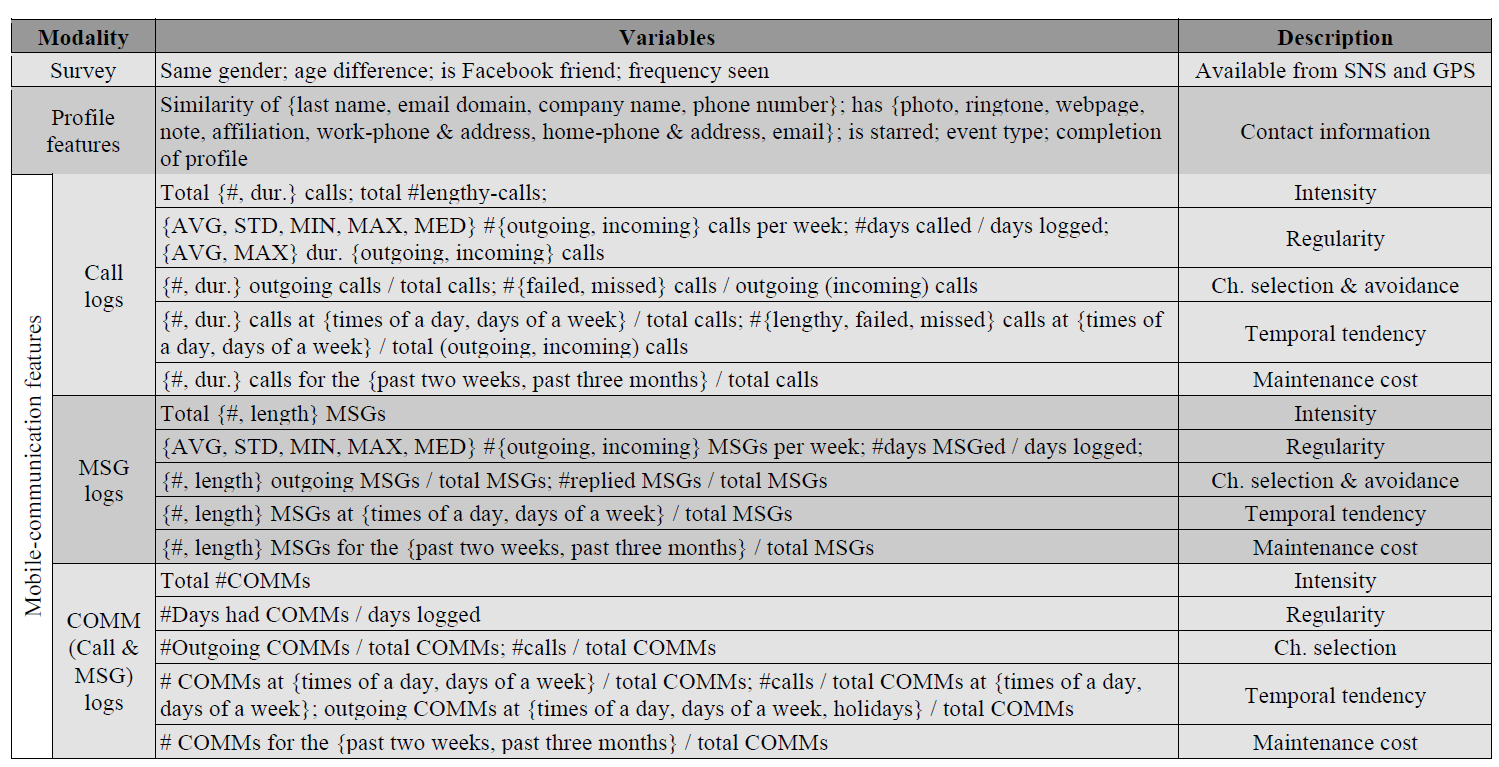
\includegraphics[width=\textwidth]{figures/feature_extraction_placeholder.png}
    \caption{Placeholder table for feature extraction, lifted from min2013mining.}
\end{figure}

\subsection{Procedure}

\section{Results}

\subsection{Communication trends}
\begin{itemize}
    \item There is an asymmetry in call in/out that is not present in sms in/out
\end{itemize}
\begin{figure}[H]
    \centering
    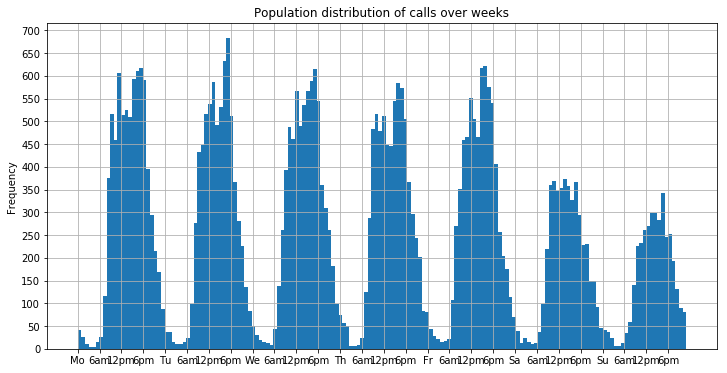
\includegraphics[width=\textwidth]{figures/call_trend.png}
    \caption{Placeholder figure for communication patterns over weeks. We likely want a plot like this, except outlier corrected (show a single representative participant?) and illustrating the different relationship types.}
\end{figure}

\begin{figure}[H]
    \centering
    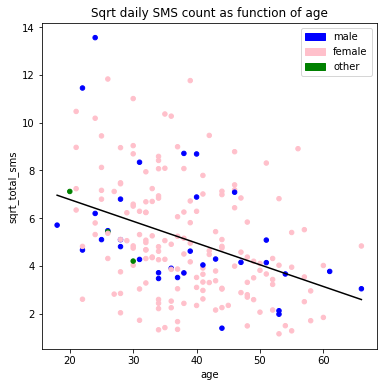
\includegraphics[width=0.5\textwidth]{figures/sms_age_scatter.png}
    \caption{Placeholder figure for communication patterns over demographics. Not sure if this plot should be included in final version, but we probably want something illustrating we took demographics into account.}
\end{figure}

\subsection{Mood disorder correlations}

\begin{figure}[H]
    \centering
    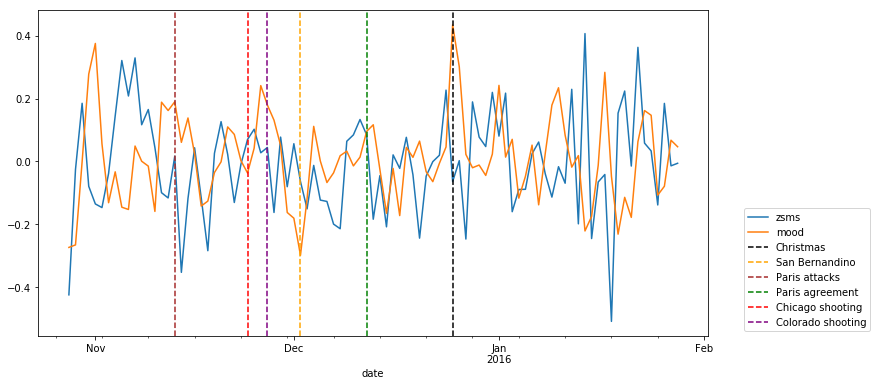
\includegraphics[width=\textwidth]{figures/sms_mood_time.png}
    \caption{Placeholder figure for exploring wellbeing vs communication relationship. Could generate a similar time plot, with anxious/depressed participants broken out into separate trend lines.}
\end{figure}
\subsection{Relationship classification}

\textbf{Contact types}
\begin{itemize}
    \item Significant Other
    \item Friend
    \item Family Member You Live With
    \item Family Member You Don't Live With 
    \item Colleague/Work-Related
    \item Task (e.g. Make an Appointment, Reservation, etc.)
\end{itemize}

Each participant is a data point, as we want to cross validate over people.

A representative loss function:

$$
\sum_{i\in\text{egos}} \frac{1}{|\text{alters}_i|} \sum_{j \in \text{alters}_i} \mathbf{1}\{\hat{y}_j \ne y_j\}
$$

Potential directions:
\begin{itemize}
    \item Auto-ML
    \item Block regularization
    \item Multi-task learning
\end{itemize}



\section{Discussion}

\subsection{Findings}

\subsection{Future work}
\nocite{*}
\bibliographystyle{plain}
\bibliography{references}
\end{document}